\documentclass{revtex4}
\usepackage{amsmath}
\usepackage{graphicx}
\usepackage{hyperref}
\begin{document}
\title{Lecture notes on probability and statistics relevant to experiments in PHYS 2501W}
\author{Prof. Andrew Puckett}
\affiliation{Dept. of Physics, University of Connecticut}
\date{\today}
\maketitle
\section{Definition of Probability Distribution, Mean, and Variance}
For a continuous random variable $x$, we define the probability density function or distribution $P(x)$ such that $\int_a^b P(x) dx$ is the probability that $x$ lies between $a$ and $b$. $P(x)$ is normalized so that its integral over all possible values of $x$ is one:
\begin{eqnarray}
  \int_{-\infty}^{\infty} P(x) dx = 1
\end{eqnarray}
We define the \emph{expectation value} of a function or operator $\mathcal{O}(x)$ as 
\begin{eqnarray}
  \left<\mathcal{O}(x) \right> &=& \int_{-\infty}^{\infty} \mathcal{O}(x) P(x) dx
\end{eqnarray}
We define the mean $\mu$ and the variance $\sigma^2$ of $x$ as 
\begin{eqnarray}
  \mu &=& \left<x\right> = \int_{-\infty}^\infty x P(x) dx \nonumber \\
  \sigma^2 &=& \left<(x-\mu)^2\right> = \int_{-\infty}^{\infty} (x - \mu)^2 P(x) dx \nonumber \\
  &=& \int_{-\infty}^{\infty} (x^2 - 2\mu x + \mu^2) P(x) dx = \left<x^2\right> - \left<x\right>^2
\end{eqnarray}
\section{Sampling statistics}
In experimental physics, we will often perform repeated measurements
of a quantity that is expected to have the same true value in each measurement, in order
to obtain an estimate of the uncertainty in the quantity, and to
reduce the uncertainty in that quantity by averaging several
independent measurements. In any individual measurement, the observed
value $x_{obs}$ will differ from the \emph{unknown} ``true'' value $x_t$
by an unknown amount $d_x = x_{obs} - x_t$. We can think of $x_{obs}$
as a random variable sampled from a probability distribution with mean
$\mu = x_t$ and standard deviation $\sigma$ characterizing the typical
error in a single measurement. Assuming
that our measurements are \emph{unbiased}, the theoretical mean of the
distribution of $x_{obs}$ is $\lim_{N \rightarrow \infty}
\left<\frac{1}{N} \sum_{i=1}^N x_i \right> = \mu = x_t$. In other words, we assume that we are
equally likely to err in either direction. Assume we have sampled the distribution of $x$ values by
performing $N$ measurements $x_i$ for $i=1,\ldots,N$. We define the \emph{sample mean} $\bar{x}$ and the \emph{sample variance} $s^2$ as 
\begin{eqnarray}
  \bar{x} &=& \frac{1}{N} \sum_{i=1}^{N} x_i \label{samplemean} \\
  s^2 &=& \frac{1}{N} \sum_{i=1}^{N} (x_i - \bar{x})^2 = \frac{1}{N} \sum_{i=1}^N x_i^2 -\frac{2}{N} \sum_{i=1}^{N} x_i \bar{x} + \frac{1}{N} \sum_{i=1}^N \bar{x}^2 \nonumber \\
  s^2 &=& \overline{x^2} - \bar{x}^2 \label{samplevariance},
\end{eqnarray}
where on the last line we have used the fact that
$\sum_{i=1}^N \bar{x}^2 =  N\bar{x}^2$ and
$\frac{-2}{N}\sum_{i=1}^N x_i \bar{x} = -2\bar{x}^2$. It follows from
the assumption of unbiased measurements that the expectation value of
the sample mean is simply the ``true'' value $x_t = \mu$. Second, let us
consider the variance of the sample mean. Since the expectation value
of the mean (the ``average of the average'') is $\mu$, the variance of
the sample mean is simply the average squared deviation of the mean of a sample of
size $N$ from the ``true'' value $\mu$:
\begin{eqnarray}
  \sigma_{\bar{x}}^2 &=& \left<(\bar{x} - \mu)^2 \right>
\end{eqnarray}
Let $d_i = x_i - \mu$ be the ``true error'' in a single measurement,
and let $D = \bar{x} - \mu$ be the ``true error'' in the sample mean. Then
$d_i - D = x_i - \bar{x}$ by definition.

The variance of the sample mean is evaluated by averaging $D^2$ over
the distribution of $x$:
\begin{eqnarray}
  \sigma^2_{\bar{x}} &=& \left<D^2\right> \nonumber \\
  &=& \left<\left(\frac{1}{N} \sum_{i=1}^N x_i - \mu\right)^2\right>
  \nonumber \\
  &=& \frac{1}{N^2}\left<\left(\sum_{i=1}^N x_i - N\mu \right)\left(\sum_{j=1}^N
      x_j - N\mu \right)\right> \nonumber \\
  &=& \frac{1}{N^2} \left<\left(\sum_{i=1}^N (x_i - \mu) \right)\left(\sum_{j=1}^N
      (x_j - \mu) \right) \right>\nonumber \\
  \sigma^2_{\bar{x}} &=& \frac{1}{N^2} \left<\sum_{i=1}^N d_i^2 +
    \sum_{i=1}^N \sum_{j \ne i}^N d_i d_j \right>  = \frac{\sigma^2}{N} \label{varianceofsamplemean},
\end{eqnarray}
where on the last line, we have replaced $(x_i - \mu)$ with $d_i$. Consider what happens when we take the expectation value in
Eq.~\eqref{varianceofsamplemean}. The expectation value of the ``true
error'' $d_i$ is zero by the assumption of unbiased
measurements. The second term inside the $\left<\ldots \right>$ in
Eq.~\eqref{varianceofsamplemean} vanishes because each of the $N$
measurements in each sample is assumed to be independent; i.e., the
error $d_i$ is uncorrelated with the error $d_j$ for $i \ne
j$. When we average this term over the distribution of a large number
of $N$-samplings, we get zero. Therefore, we are left with the term $\frac{1}{N^2}
\left<\sum_{i=1}^N d_i^2 \right>$. The expectation value
$\left<\sum_{i=1}^N d_i^2\right>$ just gives $N \left<d^2\right> = N
\sigma^2$, because each sample gives $N$ random $d^2$ values, and
the average of $d^2$ over the distribution is just $\sigma^2$, by
definition. We have thus arrived at the famous result that the
variance of the sample mean equals the variance of the parent distribution
divided by the number of measurements in the sample. Thus, if the
standard deviation $\sigma$ of the distribution of $x$ serves as a
measure of the error in a single measurement, then $\sigma_{\bar{x}}
= \sigma/\sqrt{N}$ serves as a measure of the error in the average
of $N$ independent measurements of the same quantity.

Let us consider next the relationship between the sample variance and
the distribution variance. The
expectation value of the sample variance is given by
\begin{eqnarray}
  \left<s^2 \right> &=& \frac{1}{N} \left<\sum_{i=1}^N (x_i -
    \bar{x})^2 \right> = \frac{1}{N} \left<\sum_{i=1}^N (d_i -D)^2
  \right> \nonumber \\
  &=& \frac{1}{N} \left<\sum_{i=1}^N \left( d_i^2 + D^2 - 2d_i D
    \right)\right> \nonumber \\
  &=& \sigma^2 + \frac{\sigma^2}{N} - \frac{2}{N} \left<\sum_{i=1}^N
    (x_i-\mu)(\bar{x}-\mu)\right> = \sigma^2 + \frac{\sigma^2}{N} -
  \frac{2}{N} \left<N (\bar{x}-\mu)^2 \right> \nonumber \\
  &=& \sigma^2 + \frac{\sigma^2}{N} - \frac{2}{N}\left<N D^2 \right> =
  \sigma^2 - \frac{\sigma^2}{N} = \sigma^2 \frac{N-1}{N} 
\end{eqnarray}
We therefore see that the sample variance is a \emph{biased} estimator for the
variance of the distribution, and tends to underestimate the variance
at small values of $N$. As $N$ becomes large, however, the factor
$(N-1)/N$ multiplying $\sigma^2$ tends toward one. Moreover, we see
that $s^2 \frac{N}{N-1} = \frac{1}{N-1}\sum_{i=1}^N (x_i - \bar{x})^2$
is an \emph{unbiased} estimator for $\sigma^2$.
\section{Special Probability Distributions: Binomial, Poisson and
  Gaussian}
\subsection{Binomial}
The binomial distribution describes the probability distribution of outcomes of
binary (success/failure) experiments. Specifically, the probability
$P(k)$ of observing $k$ ``successes'' in $N$ independent trials when the
probability of success is $p$ is given by:
\begin{eqnarray}
  P(k) &=& \frac{N!}{k!\left(N-k\right)!} p^k (1-p)^{N-k} \label{binomialdist}
\end{eqnarray}
The various factors appearing in Eq.~\eqref{binomialdist} are
intuitively simple to understand. The factor $p^k$ represents the product of the
individual probabilities of each of the $k$ successes. The factor
$(1-p)^{N-k}$ represents the product of the individual probabilities
for each of the $N-k$ failures. However, we don't care about the order
in which the successes and failures occur, so we have to multiply this
probability by the number of possible ways of choosing $k$ successes
from $N$ trials. It is a well-known fact that the number of possible
orderings of $N$ trials, regardless of success or failure, is
$N!$. Let $M$ be the number of possible orderings of $k$ successes
drawn from among $N$ trials. There are $N$ ways to choose the first
(successful) trial. For each possible choice of the first trial, there
are $N-1$ ways to choose the second trial, and so on all the way up to $N - k + 1$ ways to choose
the $k^{th}$ trial: 
\begin{eqnarray}
  M &=& N (N-1) (N-2) \ldots (N-k + 1) = N (N-1) (N-2) \ldots (N-k +
  1) \times \frac{(N-k)!}{(N-k)!} = \frac{N!}{(N-k)!}
\end{eqnarray}
Recalling that we don't care about the ordering of the $k$ successes,
the number of ways of choosing $k$ successes from $N$ trials is simply
given by $M/k! = \frac{N!}{k!(N-k)!}$.

\begin{figure}[h]
  \begin{center}
    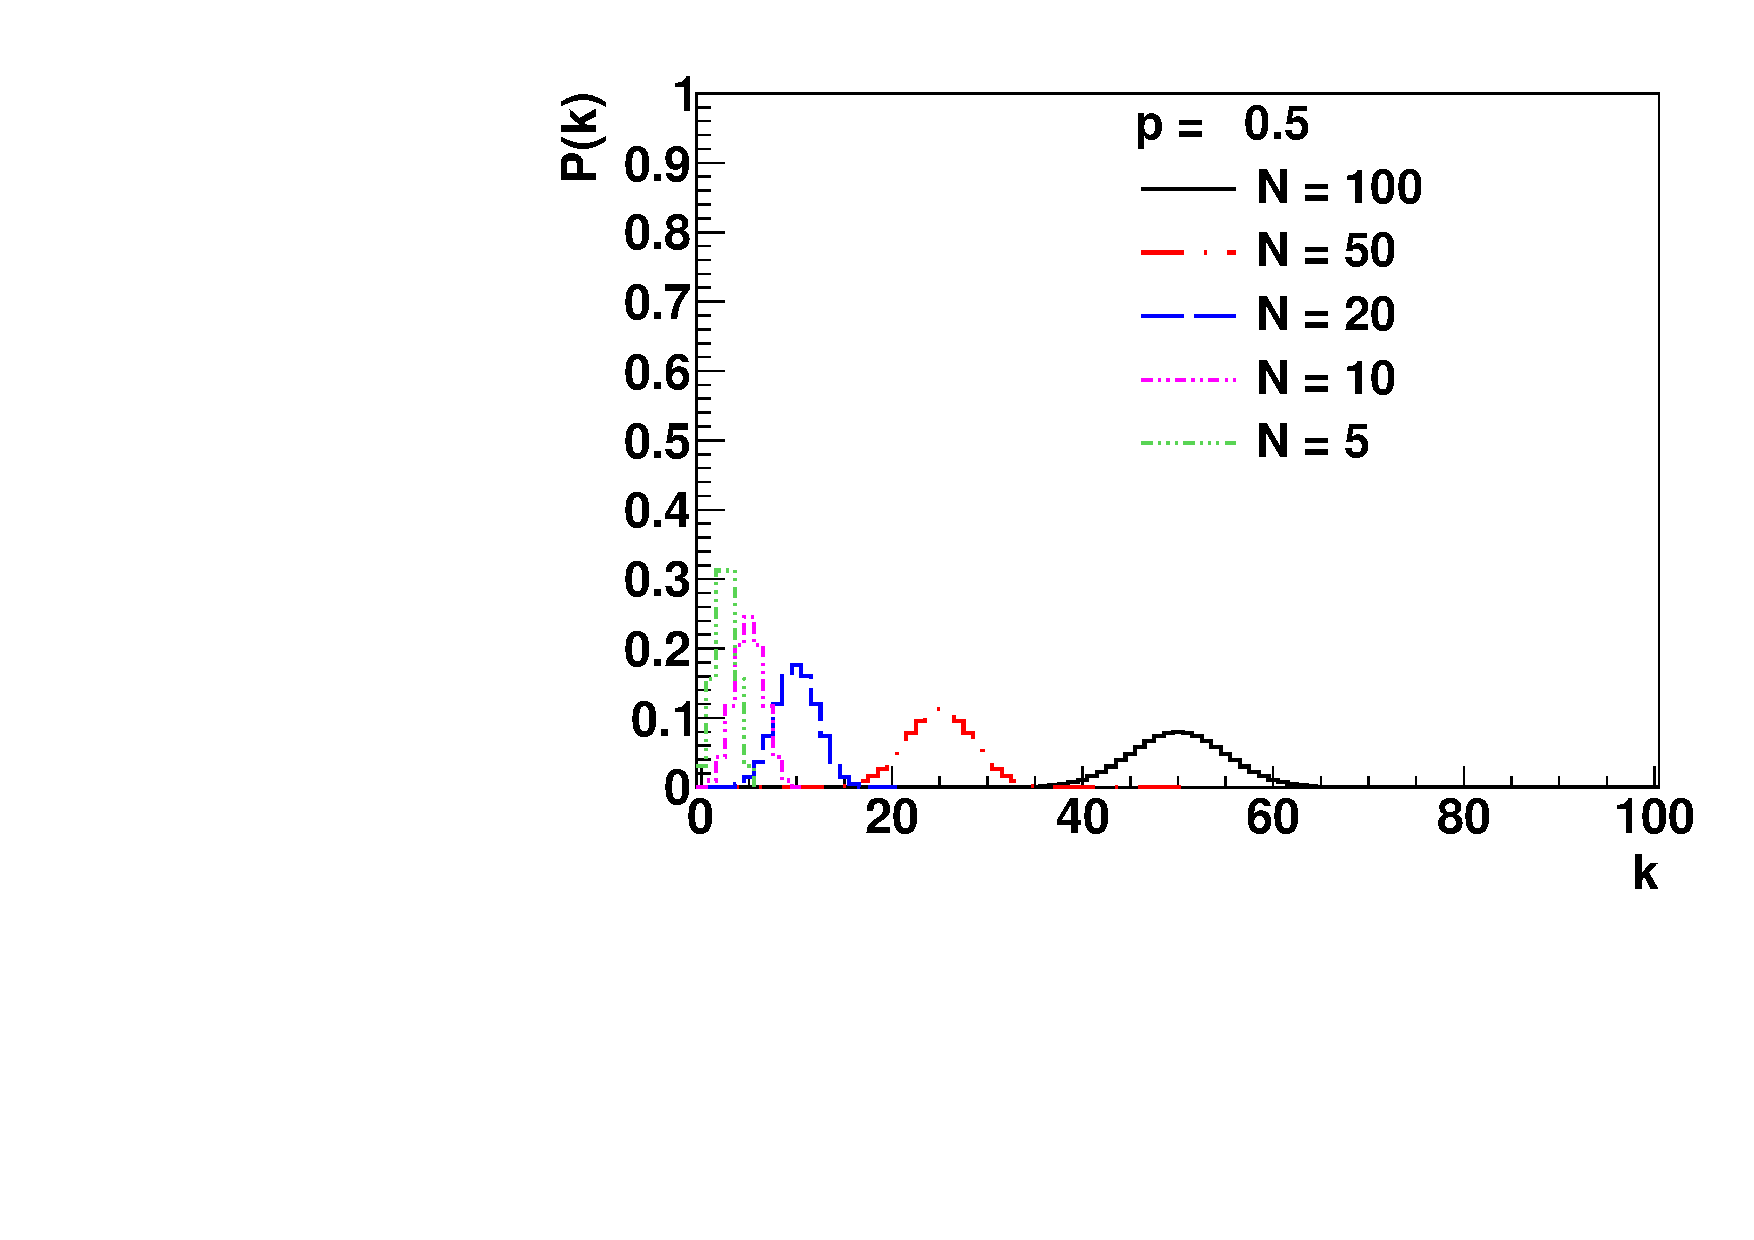
\includegraphics[width=0.48\textwidth]{Binomial_vs_N_p50.pdf}
    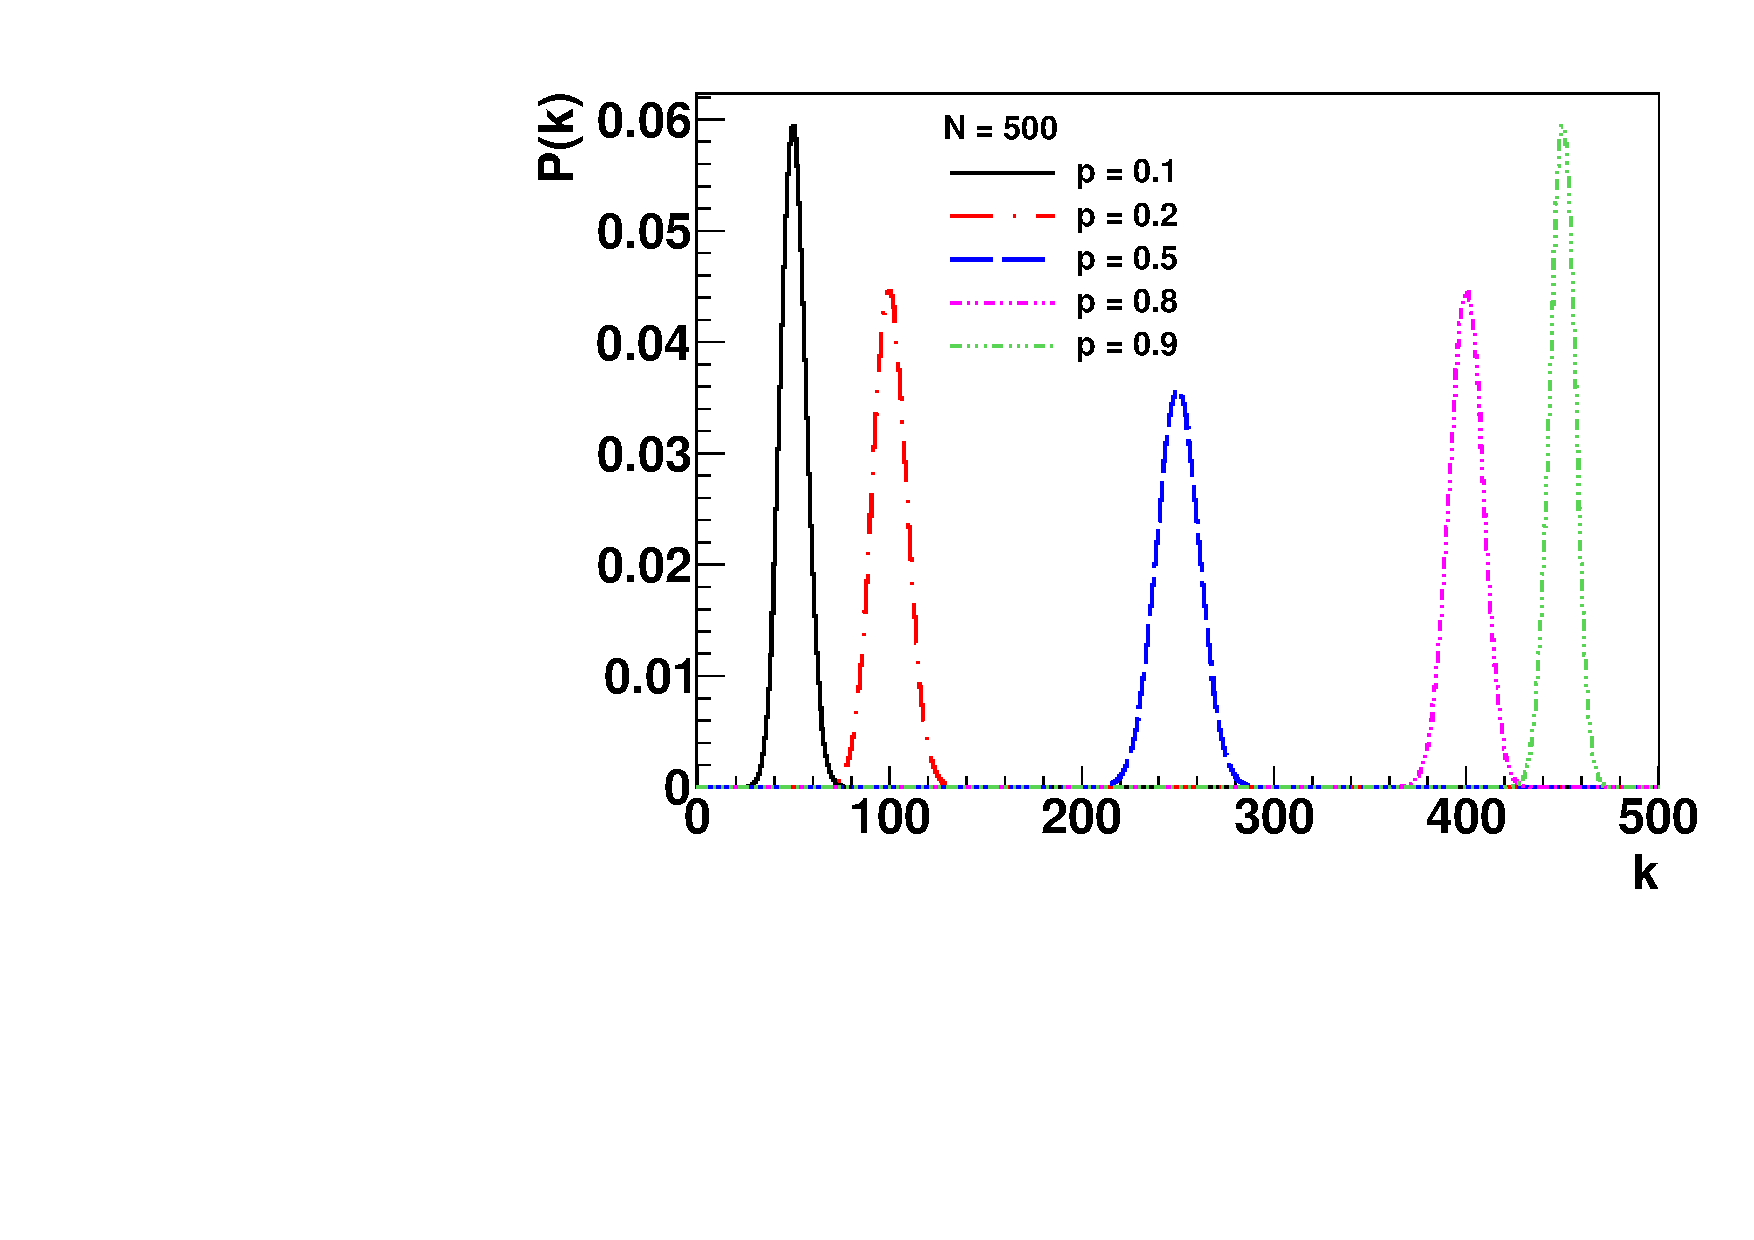
\includegraphics[width=0.48\textwidth]{Binomial_vs_p_N500.pdf}
  \end{center}
  \caption{\label{fig:binomial} Left: Binomial distribution at
    different values of $N$ for a fixed $p=0.5$. Right: Binomial
    distribution at different values of $p$ for a fixed $N = 500$.}
\end{figure}
Figure \ref{fig:binomial} shows the behavior of the binomial
distribution $P(k)$ as a function of $N$ for fixed $p$, and as a
function of $p$ for fixed $N$. We see that the average and most
probable value of $k$ is $Np$, and that the fractional deviations of
$k$ from $Np$ decrease as $N$ increases. A more quantitative statement
of this observation will be made below. The binomial distribution can be shown to be normalized (i.e., that
$\sum_{k=0}^N P(k) = 1$) by simply recognizing the fact that this sum
is equivalent to the binomial expansion of $((1-p)+p)^N = 1$. Indeed,
this is where the name ``Binomial'' distribution comes from. The mean of the binomial distribution is given by $\left<k\right> =
Np$. This can be shown by carrying out the sum of $k P(k)$ over all
$k$ from 0 to N:
\begin{eqnarray}
  \left<k\right> &=& \sum_{k=0}^N k P(k) \nonumber \\
  &=& \sum_{k=0}^N k \frac{N!}{k! (N-k)!} p^k (1-p)^{N-k} \nonumber \\
  &=& \frac{p}{1-p} \sum_{k=1}^N \frac{N!(N-k+1)}{(k-1)! (N-k+1)!} p^{k-1}(1-p)^{N-k+1} \nonumber \\
  &=& \frac{p}{1-p} \sum_{k=0}^{N-1} (N-k) P(k) = \frac{p}{1-p}
  \left[N\sum_{k=0}^{N-1} P(k) - \sum_{k=0}^{N-1} k P(k)\right]
  \nonumber \\
  \left<k\right> &=& \frac{p}{1-p}\left[N(1-p^N) - \left<k\right> + N p^N \right] =
  \frac{p}{1-p}(N-\left<k\right>) \nonumber \\
  \left(1-p+p\right)\left<k\right> = \left<k\right> &=& Np \label{binomial_mean}
\end{eqnarray}
The variance of the binomial distribution is given by $\sigma_k^2 =
Np(1-p)$, as is shown by computing the sum of $(k-Np)^2 P(k)$ over all $k$:
\begin{eqnarray}
  \sigma_k^2 + (Np)^2 &=& \sum_{k=0}^N k^2 P(k) \nonumber \\
  &=& \sum_{k=1}^N k \frac{N!}{(k-1)! (N-k)!} p^k(1-p)^{N-k} \nonumber
  \\
  &=& \frac{p}{1-p}\sum_{k=1}^N k\frac{N! (N-k+1)}{(k-1)!(N-k+1)!}
  p^{k-1}(1-p)^{N-k+1} \nonumber \\
  &=& \frac{p}{1-p} \sum_{k=1}^N k (N-k+1) P(k-1) =
  \frac{p}{1-p}\sum_{k=0}^{N-1} (k+1)(N-k) P(k) \nonumber \\
  &=& \frac{p}{1-p} \left[N \sum_{k=0}^{N-1} kP(k) + N
    \sum_{k=0}^{N-1} P(k) - \sum_{k=0}^{N-1} k^2 P(k) -
    \sum_{k=0}^{N-1} k P(k) \right] \nonumber \\
  &=& \frac{p}{1-p} \left[N( Np - Np^N) + N - Np^N - \left<k^2\right>
    + N^2 p^N - Np + Np^N \right] \nonumber \\
  &=& \frac{p}{1-p}\left[N^2 p  + N - \left<k^2\right> - Np  \right] =
  \frac{p}{1-p}\left[N(Np + 1 - p) - \left<k^2\right> \right]
  \nonumber \\
  \left<k^2\right> &=& Np(Np + 1 - p) = (Np)^2 + Np(1-p) \nonumber \\
  \Rightarrow \sigma_k^2 &=& Np(1-p)
\end{eqnarray}
The standard deviation $\sigma_k$ of $k$ is then given by 
\begin{eqnarray}
  \frac{\sigma_k}{\left<k\right>} &=& \frac{\sqrt{Np(1-p)}}{Np} = \sqrt{\frac{1-p}{Np}}
\end{eqnarray} 
Therefore we see that at fixed $p$, the fractional spread of $k$ about
the mean $Np$ decreases as $1/\sqrt{N}$ as $N$ becomes large.
\subsection{Poisson}
The Poisson distribution emerges from consideration of the Binomial
distribution in the limit as $N \rightarrow \infty$ and $p \rightarrow
0$ while the product $Np = \lambda$ remains finite, approaching a
constant value $\lambda$. A good example of a physical system governed
by Poisson statistics is a sample of low-level, long-lived radioactive
material such as $^{238}$U. The lifetime of $^{238}$U is long enough
that the number of nuclei present does not change by a measurable
amount over any reasonable time interval we can observe in the
lab. Therefore, the counting rate $R = dN/dt$, the number of decays
observed per unit time, is constant to a very good approximation.  When we observe the activity level of such
a source using a Geiger counter to count the number of decays in a
time interval $T$, the probability of any individual nucleus decaying
is very small (close to zero), whereas the number of unstable nuclei
in the sample is large, such that the expected average number of counts
$\lambda = RT$ is finite. Consider Eq.~\eqref{binomialdist} in the
limit of large $N$ and small $p$, with $Np = \lambda = $ constant. 
\begin{eqnarray}
  \lim_{N \rightarrow \infty, Np \rightarrow \lambda}
  \frac{N!}{k!(N-k)!} p^k (1-p)^{N-k} &=& \lim_{N \rightarrow
    \infty,Np \rightarrow \lambda} \frac{N(N-1)(N-2)\ldots
    (N-k+1)(N-k)!}{k!(N-k)!}p^k(1-p)^{N-k} \nonumber \\
  &=& \frac{(Np)^k}{k!} \lim_{N\rightarrow \infty, Np \rightarrow \lambda} (1-p)^{N-k} =
  \frac{\lambda^k}{k!} \lim_{N\rightarrow \infty, Np\rightarrow \lambda} (1-p)^N \nonumber \\
 \ln \left((1-p)^N\right) = N \ln (1-p) &\xrightarrow[p \rightarrow 0]{}& -Np = -\lambda \nonumber \\
 \Rightarrow \lim_{N\rightarrow \infty,Np\rightarrow \lambda} P(k) &=&
 \frac{\lambda^k e^{-\lambda}}{k!} \label{PoissonDist}
\end{eqnarray}
The discrete probability distribution represented by
Eq.~\eqref{PoissonDist} is known as the Poisson distribution. The mean
and variance of the Poisson distribution can be computed as follows:
\begin{eqnarray}
\end{eqnarray}
\subsection{Gaussian}
\section{The Central Limit Theorem}
\section{The $\chi^2$ distribution, the Least-Squares method, and the
  meaning of $\chi^2$ as a test of goodness-of-fit}

\end{document}
